% Chapter Template

\chapter{Ensayos y resultados} % Main chapter title

\label{Chapter5} 


%----------------------------------------------------------------------------------------
%	SECTION - PRUEBAS FUNCIONALES
%----------------------------------------------------------------------------------------
\section{Pruebas funcionales}
\label{sec:pruebas}
En esta sección se mencionan las pruebas funcionales unitarias realizadas sobre los diferentes puntos del proyecto.

%----------------------------------------------------------------------------------------
%	SUBSECTION - PRUEBAS FUNCIONALES DEL HARDWARE
%----------------------------------------------------------------------------------------
\subsection{Pruebas funcionales del hardware}
\label{sec:pruebasHW}

\subsubsection{Sensor temperatura DS18B20}
En esta sección se describe el banco de pruebas utilizado y la conexión del sensor DS18B20 al microcontrolador ESP32, detallando su configuración eléctrica y las consideraciones de hardware necesarias.

\subsubsection{Banco de pruebas}
Para realizar las pruebas se utilizaron los siguientes componentes:
\begin{itemize}
    \item Sensor de temperatura DS18B20.
    \item Placa de desarrollo ESP32.
    \item Resistencia de 4.7k$\Omega$.
    \item Cables de conexión.
    \item \textit{Protoboard}.
\end{itemize}

\subsubsection{Conexión del Sensor DS18B20 a la ESP32}
El DS18B20 tiene tres pines: VCC, GND y DATA. El pin DATA utiliza un protocolo 1-Wire para la comunicación con la ESP32, por lo que solo necesita un pin de entrada/salida en el PCB. La conexión se realizó de la siguiente manera:

\begin{itemize}
    \item VCC del DS18B20 conectado a 5 V.
    \item GND del DS18B20 conectado a GND .
    \item DATA del DS18B20 conectado al pin GPIO17 de la ESP32.
    \item Se utilizó una resistencia de 4.7k$\Omega$ entre VCC y el pin DATA para asegurar la correcta comunicación, tal como lo indica la hoja de datos del fabricante \citep{Sensor_temp}.
\end{itemize}

La figura \ref{fig:conexionTemperatura} muestra el diagrama de conexión del sensor DS18B20 a la ESP32.

\begin{figure}[h]
    \centering
    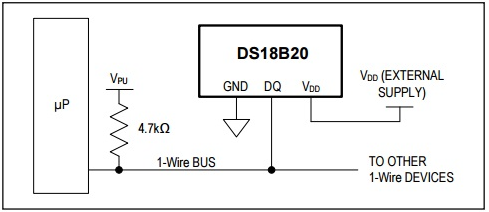
\includegraphics[width=0.8\textwidth]{./Figures/Pruebas/conexion_ds18b20.png}
    \caption{Conexión del sensor DS18B20 a la ESP32.}
    \label{fig:conexionTemperatura}
\end{figure}

\subsubsection{Código Implementado}
El código se escribió utilizando el entorno de desarrollo VisualStudio 2022, con la biblioteca nanoFramework.Device.OneWire para la comunicación del sensor y la biblioteca Iot.Device.Ds18b20 para la lectura de los datos de temperatura. El siguiente fragmento de código \ref{codigoDS18B20} se empleo para el desarrollo de la prueba:
\begin{lstlisting}[language=C, label=codigoDS18B20, caption= Fragmento del código del sensor de temperatura DS18B20]

using Iot.Device.Ds18b20;
using nanoFramework.Device.OneWire;

        private void ConfigurarSensorTemperatura()
        {
            Configuration.SetPinFunction(16, DeviceFunction.COM3_RX);
            Configuration.SetPinFunction(17, DeviceFunction.COM3_TX);

            OneWireHost oneWire = new OneWireHost();


            ds18b20 = new Ds18b20(oneWire, null, false, TemperatureResolution.VeryHigh);

            ds18b20.IsAlarmSearchCommandEnabled = false;
            if (ds18b20.Initialize())
            {
                Console.WriteLine($"Is sensor parasite powered?:{ds18b20.IsParasitePowered}");
                string devAddrStr = "";
                foreach (var addrByte in ds18b20.Address)
                {
                    devAddrStr += addrByte.ToString("X2");
                }

                Console.WriteLine($"Sensor address:{devAddrStr}");
            }
        }

                private double MedirTemperatura()
        {
            if (!ds18b20.TryReadTemperature(out var currentTemperature))
            {
                Console.WriteLine("Can't read!");
                return -1;
            }
            else
            {
                Console.WriteLine($"Temperature: {currentTemperature.DegreesCelsius.ToString("F")}\u00B0C");
                return currentTemperature.DegreesCelsius;
            }
        }
\end{lstlisting}

\subsubsection{Resultados de las Pruebas}
Las pruebas se realizaron en condiciones de laboratorio. Para ello se introdujo el sensor en una maceta con tierra y arena (simulando las condiciones de trabajo real) y se agregó agua caliente para variar la temperatura del suelo. Se usó un termómetro digital para comparar las lecturas de temperatura \citep{Magesa} y validar el funcionamiento del sensor de temperatura DS18B20.

Se observaron los siguientes resultados:
\begin{itemize}
    \item El sensor DS18B20 se conectó exitosamente a la placa ESP32, siguiendo el esquema de conexión descrito.
    \item La comunicación entre el sensor y la ESP32 fue estable gracias a la resistencia de pull-up de 4.7k$\Omega$ entre VCC y DATA.
    \item Las lecturas de temperatura fueron consistentes y precisas en un rango de 10°C a 80°C, mostrando una precisión dentro de ±0.5°C, que es lo esperado para este sensor.
    \item Los resultados se imprimieron en el monitor serial, actualizándose cada segundo.
    \item Las condiciones de humedad no afectaron ni destruyeron al sensor, comprobando su capacidad de sumergible.
\end{itemize}

\subsubsection{Conclusiones}
El sensor de temperatura DS18B20 es una solución efectiva para medir temperaturas con precisión y simplicidad, utilizando una única línea de datos para la comunicación con la ESP32. Las pruebas realizadas confirmaron el correcto funcionamiento del sistema, con resultados precisos y consistentes.


\subsubsection{Sensor de Humedad YL-69}
A continuación se describen la conexión y pruebas realizadas con el sensor de humedad YL-69, que se utiliza para medir la humedad del suelo.

\subsubsection{Banco de pruebas}
Para realizar las pruebas se utilizaron los siguientes componentes:
\begin{itemize}
    \item Sensor de humedad YL-69.
    \item Módulo comparador YL-38.
    \item Placa de desarrollo ESP32.
    \item Cables de conexión.
    \item Protoboard.
    \item Fuente de alimentación de 5 V.
\end{itemize}

\subsubsection{Conexión del Sensor de Humedad YL-69 a la ESP32}
El sensor de humedad YL-69 es un dispositivo que mide la resistencia entre dos sondas insertadas en el suelo. Esta medición se traduce en un valor analógico que refleja la humedad del suelo. El sensor YL-69 funciona junto con el módulo YL-38, que convierte la señal analógica en digital para facilitar la lectura con microcontroladores.

La conexión se realizó de la siguiente manera:

\begin{itemize}
    \item VCC del YL-38 conectado a 5 V.
    \item GND del YL-38 conectado a GND.
    \item La salida analógica (A0) del YL-38 conectada al pin GPIO35 (entrada ADC) de la ESP32.
    \item Las sondas del YL-69 conectadas a los pines correspondientes del módulo YL-38.
\end{itemize}

La Figura \ref{fig:conexion_yl69} muestra el diagrama de conexión del sensor de humedad YL-69 al ESP32.

\begin{figure}[h]
    \centering
    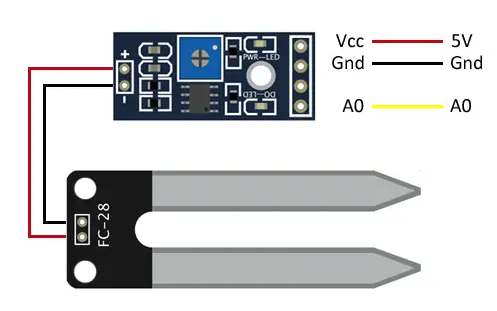
\includegraphics[width=0.8\textwidth]{./Figures/Pruebas/conexion_yl69.png}
    \caption{Conexión del sensor de humedad YL-69 al ESP32. Fuente: \citep{higrometroFC-28}.}
    \label{fig:conexion_yl69}
\end{figure}

\subsubsection{Código Implementado}
El código se escribió utilizando el mismo entorno de desarrollo que para el sensor de temperatura. El valor analógico del sensor de humedad se lee a través del puerto ADC de la ESP32.

El fragmento de código \ref{codigoYL-69} se utilizo para realizar las pruebas correspondientes.

\begin{lstlisting}[language=C, label=codigoYL-69, caption= Fragmento del código del sensor de humedad YL-69]

using System;
using nanoFramework.Hardware.Esp32;
using Windows.Devices.Adc;

        private void ConfigurarSensorHumedad()
        {
            // Configurar el pin ADC
            adc = new AdcController();

            //HUMEDAD          -----> ADC Channel 7 - GPIO 35 
            humedadAdc = adc.OpenChannel(7);

            Console.WriteLine("Sensor de humedad configurado.");
        }

         private double MedirHumedad()
        {
            
            
            int analogValue = humedadAdc.ReadValue();

            float vSensor = (analogValue / 4095f * 3.3f);
            double humidityPercentage = (-48.95 * vSensor * vSensor * vSensor) + (368.10 * vSensor * vSensor) - 910.85 * vSensor + 757.17;

            Console.WriteLine($"Analog Humedad: {analogValue}");
            Console.WriteLine($" tension: {vSensor}");
            if(humidityPercentage>100) humidityPercentage=100;
            if(humidityPercentage<0) humidityPercentage=0;

            return humidityPercentage;

        }
\end{lstlisting}

Es importante destacar que la humedad del suelo es un parámetro relativo ya que no se mide en términos absolutos (litros de agua por metro cúbico de suelo) en la mayoría de los casos, sino en relación a la capacidad del suelo para retener agua. Hay varios parámetros clave que hacen de la humedad del suelo una medida relativa, como por ejemplo la temperatura y la presión.

Es por eso que para la calibración del sensor de humedad se tuvo en cuenta un estudio\cite{yl_69_calibration} donde se comparó las mediciones del sensor con las de un método más preciso conocido como el método gravimétrico.

Con los resultados de este estudio se desarrollaron mediciones comparativas y aproximaciones polinómicas de las lecturas del ADC para obtener una fórmula que permita traducir los niveles de tensión a porcentaje de humedad. Esto dió como resultado la siguiente fórmula:

\begin{equation}
f(x) = 757.17 - 910.85x + 368.01x^2 - 48.95x^3
\end{equation}


\subsubsection{Resultados de las Pruebas}
Las pruebas se realizaron insertando las sondas del sensor YL-69 en diferentes tipos de suelos, desde secos hasta saturados de agua. Se realizaron varias mediciones y se observaron los siguientes resultados:

\begin{itemize}
    \item El sensor YL-69 se conectó exitosamente a la ESP32, y las lecturas de humedad se obtuvieron sin inconvenientes.
    \item El sensor respondió de manera eficiente a los cambios en el nivel de humedad del suelo, mostrando un aumento en los valores analógicos a medida que el suelo se humedecía.
    \item Las lecturas variaron entre un 0\% de humedad en suelo seco hasta un 100\% en suelo saturado.
    \item La estabilidad de las lecturas se mantuvo, incluso en condiciones de humedad extrema.
\end{itemize}

\subsubsection{Conclusiones}
Es importante mencionar que normalmente la manera de medir la humedad del compost se desarrolla de manera manual, tomando una cierta cantidad de compost en las manos y comprimiéndola para ver si drena agua entre los dedos y se forma una masa barrosa, o si al soltarlo el material se desparrama.

El sensor de humedad YL-69 demostró ser un instrumento eficaz para medir la humedad del suelo, proporcionando lecturas confiables en un rango amplio de condiciones. La integración con la ESP32 fue sencilla, y el uso del módulo YL-38 permitió leer tanto señales digitales como analógicas del sensor. Los resultados obtenidos en las pruebas indicaron un comportamiento estable y preciso. El método diseñado para medir la humedad permite reemplazar el trabajo manual y proveer un poco más de información sin estar presente en la zona.



\subsubsection{Panel Solar Cargador Batería 12 V 10 W}
A continuación, se describen las conexiones y pruebas realizadas con el panel solar Cargador Batería 12 V 10 W.

\subsubsection{Banco de pruebas}
Para realizar este proyecto, se utilizaron los siguientes componentes:
\begin{itemize}
    \item Panel  Solar Cargador Batería 12 V 10 W.
    \item Controlador de carga solar.
    \item Batería de 12 V.
    \item Cables de conexión.
    \item Multímetro.
\end{itemize}

\subsubsection{Conexión del Panel Solar a la Batería}
El panel Solar Cargador Batería 12 V 10 W se utilizó para cargar una batería de 12 V mediante un controlador de carga solar. La conexión se realizó de la siguiente manera:

\begin{itemize}
    \item Conectar el terminal positivo del panel solar al terminal positivo de la entrada del controlador de carga.
    \item Conectar el terminal negativo del panel solar al terminal negativo de la entrada del controlador de carga.
    \item Conectar el terminal positivo de la batería al terminal positivo de la salida del controlador de carga.
    \item Conectar el terminal negativo de la batería al terminal negativo de la salida del controlador de carga.
\end{itemize}

La Figura \ref{fig:conexionPanel} muestra el diagrama de conexión del panel solar al controlador de carga y a la batería.

\begin{figure}[h]
    \centering
    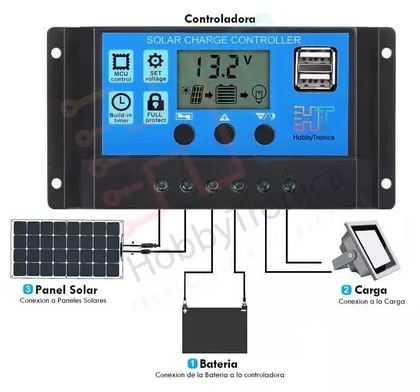
\includegraphics[width=0.8\textwidth]{./Figures/Pruebas/conexion_panel_solar.png}
    \caption{Conexión del panel Solar Cargador Batería 12 V 10 W.}
    \label{fig:conexionPanel}
\end{figure}


\subsubsection{Resultados de las Pruebas}
Las pruebas se realizaron en condiciones de iluminación natural, colocando el panel solar al aire libre. A continuación, se detallan los resultados:

\begin{itemize}
    \item El panel solar fue capaz de generar un voltaje constante en condiciones de sol pleno, alcanzando aproximadamente 14.5 V.
    \item El controlador de carga funcionó adecuadamente, regulando el voltaje y protegiendo la batería de sobrecargas.
    \item La batería se cargó satisfactoriamente, manteniendo un voltaje de alrededor de 13.8 V al finalizar la prueba.
\end{itemize}

\subsubsection{Conclusiones}
El panel solar Solar Cargador Batería 12 V 10 W es una solución adecuada para la carga de baterías de 12 V en sistemas de baja potencia. Las pruebas realizadas confirmaron su capacidad de generar energía suficiente bajo condiciones de sol pleno. Además, la integración con un controlador de carga garantiza la protección de la batería y una carga eficiente, logrando resultados estables y predecibles.

\subsection{Cálculos de alimentación Nodo Sensor}
\subsubsection{Consumos Nodo Sensor}
Para estimar el consumo y la duración de las baterías del Nodo Sensor, se buscó en las hojas de datos el consumo máximo de cada componente del sistema y se calculó el consumo total del nodo. 

En la tabla \ref{tab:consumosNodo} se notan estos valores (el consumo total se indican en mas de un renglón pero con distintas unidades).


\begin{table}[h]
    \centering

    \begin{tabular}{@{}lc@{}}
        \toprule
        \textbf{Componente}            & \textbf{Consumo (mA)} \\ \midrule
        ESP32 Wroom                   & 120 mA (promedio)      \\ 
        LoRa SX1278                   & 120 mA                  \\ 
        Sensor de temperatura DS18B20  & 1,5 mA     \\ 
        Sensor de humedad YL-69        & 20 mA                  \\ 
        Regulador Mini-360             & 90\% eficiencia                  \\ \midrule
        %\textbf{Consumo total}        & \textbf{287.65 mA}     \\ \bottomrule
        \textbf{Consumo total}        & \textbf{1438 mW}     \\ \bottomrule
    \end{tabular}
    \caption{Consumo de los componentes en mAh}
    \label{tab:consumosNodo}
\end{table}

\subsubsection{Capacidad de la pilas}
En la tabla \ref{tab:capacidadPilas} se denota la capacidad de las pilas. Para el cálculo de la capacidad efectiva de las pilas se tuvo en cuenta el nivel de tensión mínimo que el fabricante recomienda (ver sección \ref{sec:AlimentacionNodoSensor}). 

Al realizar el cálculo:
\begin{equation}
   \frac{Tension_{min} * Capacidad (Ah)}{Tension_{max}} = \frac{5.6v * 3.5Ah}{7.5v} = 2.61 Ah
\label{eq:capacidadEfectiva}
\end{equation}

Se obtiene la capacidad efectiva en Ah. Al multiplicar este valor por el valor de la tensión mínima, se obtiene la capacidad en Wh, siendo esta de 14.63 Wh.

Por último, al final de la tabla \ref{tab:capacidadPilas} se nota el tiempo de funcionamiento en horas del sistema en un régimen de trabajo de modo continuo.

\begin{table}[H]
    \centering
    \begin{tabular}{@{}lc@{}}
        \toprule
        \textbf{Especificación}       & \textbf{Valor}          \\ \midrule
       % Capacidad de las pilas      & 3.5 Ah (3500 mAh)        \\ 
        Capacidad de las pilas     & 25,9 Wh       \\ 
       % Capacidad efectiva de las pilas (Ah)      & 2,613 Ah      \\ 
        Capacidad efectiva de las pilas      & 14,63 Wh      \\ 
        Tiempo de funcionamiento & $\frac{14,63 \text{ Wh}}{1,43 \text{ w}} \approx 10,17 \text{ horas}$ \\ \bottomrule
    \end{tabular}
    \caption{Capacidad de las pilas}
    \label{tab:capacidadPilas}
\end{table}

A modo de prueba se decidió por implementar un régimen de trabajo de envío de información cada 10 segundos. Es decir, el sistema realiza una medición, envía la información sensada al Nodo AP y únicamente el ESP32 y el LoRa entran en modo Deep Sleep durante los próximos 10 segundos. Tanto los sensores de temperatura y humedad como el regulador de tensión permanecen con sus regímenes de consumo normal.

Bajo este régimen de trabajo, el sistema duró aproximadamente 21 horas operando, tal como lo indica la figura \ref{fig:PruebaBateria}.

\subsubsection{Conclusión}
Considerando que el régimen de trabajo normal es una medición por hora, es decir, una frecuencia de trabajo 360 veces más lenta que la sometida a prueba, y realizando una estimación general, se calcula que la autonomía del sistema sería aproximadamente de 7560 horas, lo que equivale a 315 días.

Teniendo en cuenta que el proceso de descomposición de la materia orgánica suele durar entre 3 y 5 meses aproximadamente (dependiendo de varios factores, como por ejemplo estación del año), se contempla que la autonomía de la batería es más que suficiente y cumple los requisitos establecidos.

\begin{figure}[H]
	\centering
	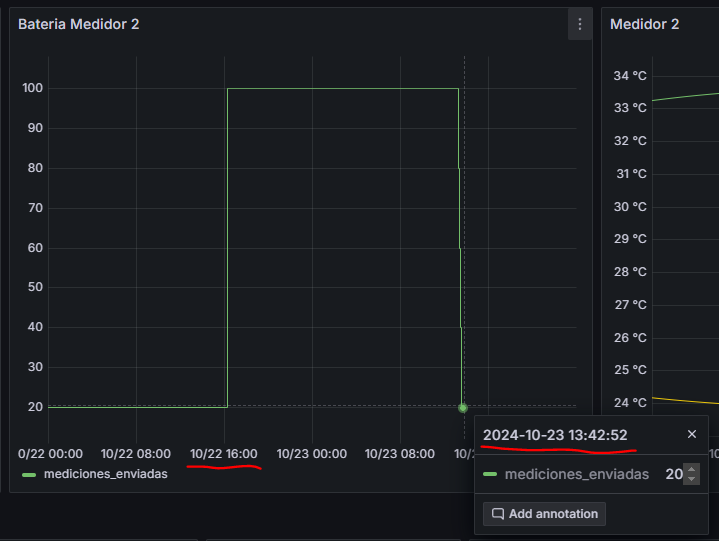
\includegraphics[scale=0.9]{./Figures/Pruebas/duracion_pila.png}
	\caption{Duración pilas - régimen de trabajo : 10 sg}
	\label{fig:PruebaBateria}
\end{figure}



\subsection{Cálculos de alimentación Nodo Access Point}
\subsubsection{Consumos componentes Nodo Access Point}

Para estimar el consumo y la duración de la batería del Nodo Access Point, se consultaron las hojas de datos para obtener el consumo máximo de cada componente del sistema y se calculó el consumo total del nodo. En la Tabla \ref{tab:consumosAP} se detallan estos valores.

\begin{table}[H]
    \centering

    \begin{tabular}{@{}lc@{}}
        \toprule
        \textbf{Componente}            & \textbf{Consumo (mA)} \\ \midrule
        ESP32 Wroom                   & 120 mA (promedio)      \\ 
        LoRa SX1278                   & 10.8 mA                  \\ 
        Router 4G portátil            & 300 mA                  \\ 
        Gerenciador                 & 10 mA                  \\ 
        Regulador Mini-360             & 90\% eficiencia                  \\ \midrule
     %   \textbf{Consumo total}        & \textbf{454 mA}     \\ \bottomrule
        \textbf{Consumo total}        & \textbf{2270 mW}     \\ \bottomrule
    \end{tabular}
    \caption{Consumo de los componentes en mAh}
    \label{tab:consumosAP}
\end{table}

Se observa una diferencia en los valores del modulo LoRa, ya que para este nodo el funcionamiento del modulo es en modo escucha y no en transmisión.

\subsubsection{Capacidad de la batería}
En la tabla \ref{tab:capacidadBat} se muestra la capacidad de la batería. Para calcular la capacidad efectiva de la batería se tomó en cuenta el nivel de tensión mínima recomendado por el fabricante. Se empleó la cuenta \ref{eq:capacidadEfectiva} dando como resultado una capacidad efectiva de 58.33 Wh.
Por último se nota que el tiempo de funcionamiento en modo continuo es de aproximadamente 25.7 horas.
\begin{table}[H]
    \centering
    \begin{tabular}{@{}lc@{}}
        \toprule
        \textbf{Especificación}       & \textbf{Valor}          \\ \midrule
       % Capacidad de la batería       & 7 Ah (7000 mAh)        \\ 
        Capacidad de la batería       & 84 Wh       \\ 
      %  Capacidad efectiva de la batería       & 5,83 Ah      \\ 
        Capacidad efectiva de la batería       & 58.33 Wh      \\ 
        Tiempo de funcionamiento  & $\frac{58.3 \text{ Wh}}{2.27 \text{ w}} \approx 25.7 \text{ horas}$ \\ \bottomrule
    \end{tabular}
    \caption{Capacidad de las baterías del Nodo Access Point}
    \label{tab:capacidadBat}
\end{table}
Para realizar la prueba de autonomía se establecieron las siguientes configuraciones:

\begin{itemize}
    \item La batería se encontraba cargada al 100\%.
    \item Se desconecto el panel solar para evitar cargar la batería.
    \item Se estableció una frecuencia de envió de métricas del Nodo Access Point al portal de 5 mins.
    \item Se estableció una frecuencia de envío de métricas del Nodo Sensor al Nodo Access Point de 10 segundos.
\end{itemize}
Bajo estas condiciones de trabajo, la autonomía del Nodo Access Point fue de 23 horas.

\subsubsection{Conclusión}
Considerando que el régimen de trabajo normal es una medición por hora y que el panel solar se encuentra conectado al sistema (aportando carga a la batería), se contempla que la autonomía de la batería es suficiente y cumple los requisitos establecidos, aunque como mejora del sistema se podría optar por una batería de una capacidad un poco mayor para tener mas autonomía. 
%----------------------------------------------------------------------------------------
%	SUBSECTION - PRUEBAS FUNCIONALES DEL FIRMWARE
%----------------------------------------------------------------------------------------
\subsection{Pruebas funcionales del firmware}
\label{sec:pruebasFW}

El objetivo de estas pruebas era determinar el correcto funcionamiento del firmware, tanto del NanoKernel, como de los Nodos Sensor y Nodo Access Point. 
Para ello se armaron pruebas incrementales, de forma tal de primero probar funcionalidades unitarias, y luego hacer pruebas integrales en un entorno local y controlado (sin uso del portal web).

Para todas estas pruebas, se utilizaron las herramientas de debugging nativas de Visual Studio 22 y la extensión de nanoframework, como también herramientas de logging en servicios web locales, y mediciones del espectro en la banda de transmisión de LoRa.

\subsubsection{Listado de pruebas}

Las pruebas fueron las siguientes:

\begin{enumerate}
    \item Correcto funcionamiento del NanoKernel.
    \item Conectividad a red Wi-Fi desde un nodo.
    \item Conexión y envío de paquetes LoRa desde un nodo.
    \item Envió de paquetes LoRa desde un nodo hacia otro.
    \item Prueba de envío de un \textit{payload} JSON desde un nodo a un servicio web en una red WiFi local.
    \item Prueba de Nodo Sensor con medición de sensores, envío de paquete LoRa, y bucle con DeepSleep.
    \item Prueba de Nodo Access Point  con simulación de paquetes LoRa entrante, manejo de colas, y envío de mediciones a servicio web en red local.
    \item Prueba de Nodo Sensor y Nodo Access Point, contra un servicio web en red local.
    \item Prueba de 2 Nodo Sensor y Nodo Access Point, contra un servicio web en red local.
    \item Prueba final de 2 Nodo Sensor y Nodo Access Point, conectados al router 4G portátil, contra un servicio en la red local expuesto a la red pública.
\end{enumerate}

Una vez realizada la prueba 10, se considera que el firmware se encuentra en condiciones de acoplarse al sistema del Portal web: como todas las pruebas se realizaron teniendo en cuenta el contrato de servicios establecido por el Portal web, la integración real consiste en simplemente un cambio de url en el endpoint.

\subsubsection{Resultados}

Entre los principales desafíos de las pruebas se encuentra el manejo de la tecnología LoRa, ya que la misma implica distintas dificultades tanto a nivel hardware como firmware.
Es por eso que para la prueba 3 no sólo se hizo uso de logeo en depuración, sino tambien de un analizador de espectro digital (SDR basado en el chip rtl2832u) para poder depurar la señal, confirmar la frecuencia de su portadora, ancho de banda, y nivel respecto al piso de ruido. Para ello se empleó la herramienta AirSpy, el cual permite observar el espectro en base al IQ enviado por USB del SDR, como se observa en la figura \ref{fig:pruebas_firmware_1}.

\begin{figure}[H]
    \centering
    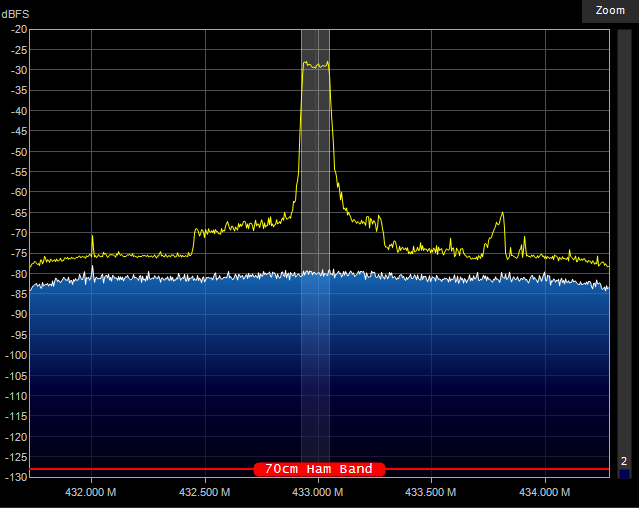
\includegraphics[width=1\linewidth]{Figures/Firmware/espectro.png}
    \caption{Análisis espectral de un emisor LoRa con la portadora en 433 MHz y 125 kHz de ancho de banda.}
    \label{fig:pruebas_firmware_1}
\end{figure}

Con esta herramienta se permitió determinar, no sólo que efectivamente el Módulo LoRa está enviando paquetes en el medio, sino también corroborar su correcta configuración de portadora y ancho de banda (entre otros). Esto es así ya que el umbral amarillo (detector de máximos) muestra que la señal LoRa se encuentra ubicada correctamente en la portadora de 433 MHz, con un ancho de banda de 125 KHz, y un nivel de la señal sobre el piso de ruido (SNR) mucho mayor a 0dB. Éste último parámetro es de vital importancia ya que indica la calidad con la que el receptor va a recibir la señal. Depende principalmente de la corriente que pueda brindar la fuente de alimentación, de la antena del Módulo LoRa, la antena del SDR, y la distancia entre las antenas. En este caso, dado que no hace falta una medición espectral absoluta ni precisa, simplemente de forma preliminar se puede observar que el Módulo LoRa opera en rangos correctos.

Por otra parte, otro de los obstáculos que se encontraron a lo largo de las pruebas fue el manejo de memoria por parte del Nodo Access Point, ya que el mismo almacena en un \textit{buffer} los mensajes encolados para enviar, por lo que es un recurso muy limitado que sobrecargaba al \textit{garbage collector}, y por ende a la CPU.

Dado que todas las pruebas se realizaron en modo depuración, fue de vital importancia tener registro de la memoria total, memoria liberada, cantidad de paquetes encolados, paquetes enviados, paquetes perdidos, la cantidad de errores, etc, y así poder describir al sistema con el fin de parametrizar la configuración y conseguir el mayor throughput con la menor tasa de error posible. En la Figura \ref{fig:pruebas_firmware_2} se observa un extracto de los logs del Nodo AP:

\begin{figure}[H]
    \centering
    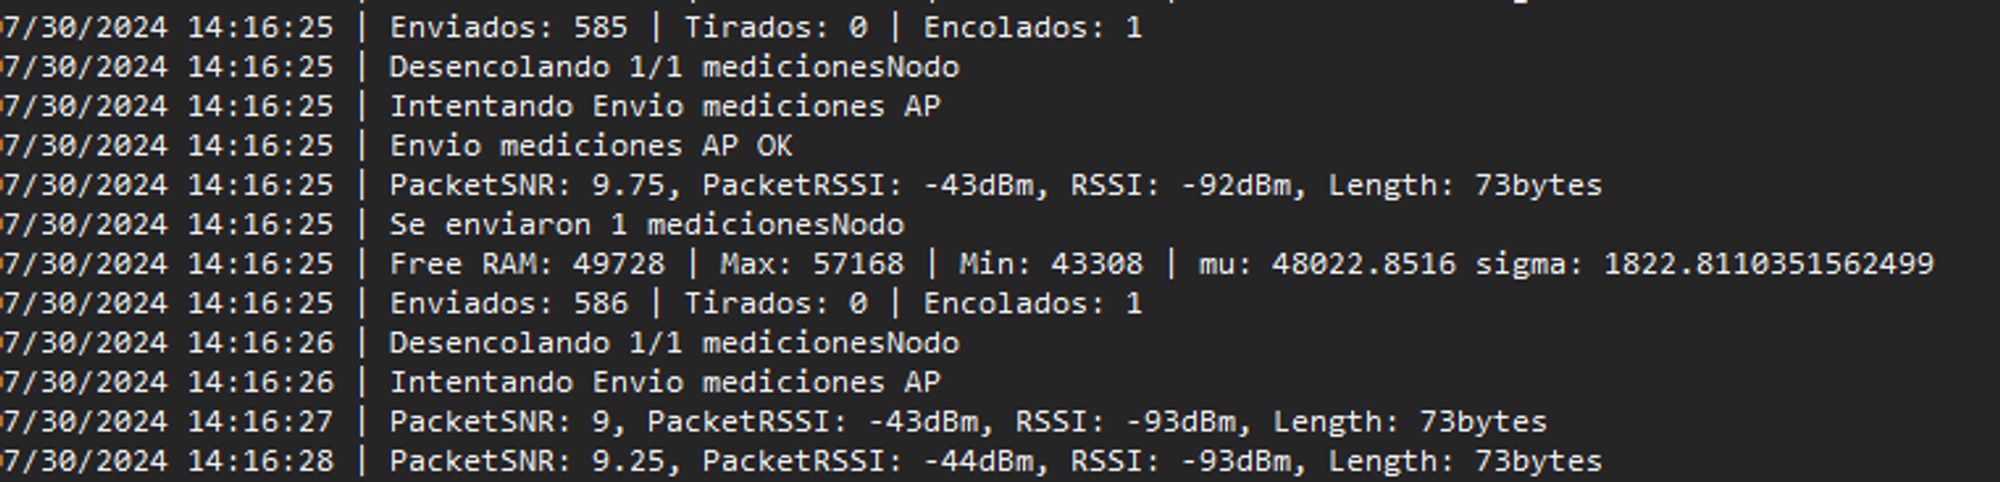
\includegraphics[width=1\linewidth]{Figures/Firmware/pruebas_2.png}
    \caption{Ejemplo captura de logging del Nodo Access Point.}
    \label{fig:pruebas_firmware_2}
\end{figure}

Para el monitoreo de memoria y cuantización de paquetes y errores se utilizó una herramienta ad hoc de muestreo de valores, el cual registra la cantidad de mediciones, el máximo, mínimo, promedio y desvío estándar.

\begin{figure}[H]
    \centering
    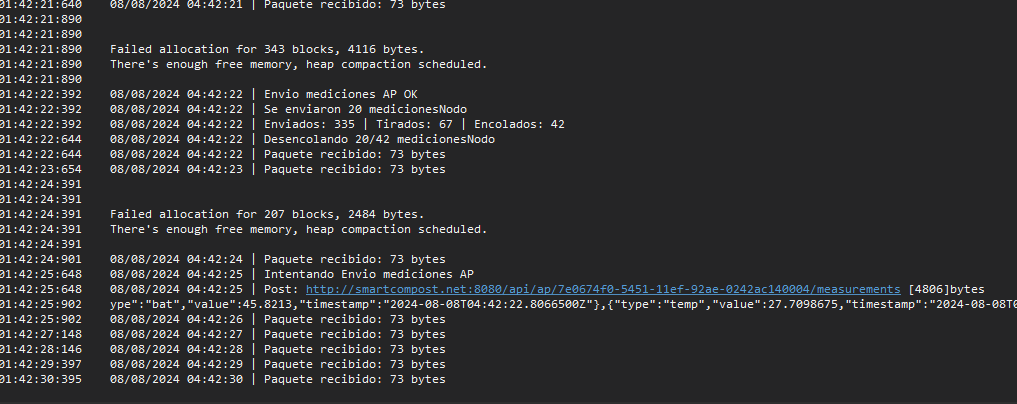
\includegraphics[width=1\linewidth]{Figures/Firmware/pruebas_1.png}
    \caption{Captura de logging del Nodo Access Point de un \textit{hit} del \textit{garbage collector}.}
    \label{fig:pruebas_firmware_1}
\end{figure}

 En la Figura \ref{fig:pruebas_firmware_1} se observa también el hit del garbage collector, mostrando la cantidad de memoria liberada, como también el JSON enviado al Portal Web, y distintos mensajes LoRa recibidos con el tamaño (en nuestro caso fijo de 73 bytes).


Cabe destacar que el propio logueo sobrecarga a la CPU, y por lo tanto cuando se compila en modo \textit{Release} (productivo), los mismos no ocurren y así se libera carga.

Por último, las pruebas finales se utilizaron para afinar los parámetros del Nodo Access Point, como el tamaño de la cola, tiempo de envío, etc, ya que el sistema en cuestión depende mucho de la velocidad de envío HTTP, haciendo que cualquier retardo en la cola, ésta se acumule y desborde, perdiendo efectivamente paquetes: lo que se buscó fue minimizar la taza de pérdida de paquetes en condiciones reales.

Los siguientes parámetros de la configuración del Nodo AP fueron los resultantes luego de varias iteraciones:

\begin{figure}[H]
    \centering
    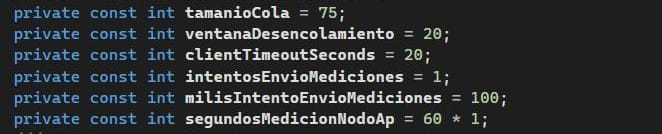
\includegraphics[width=1\linewidth]{Figures//Firmware/configuracion_tuneada.png}
    \caption{Configuración del Nodo AP óptima para red móvil 4G.}
    \label{fig:enter-label}
\end{figure}

Con ello se consiguió una tasa de error menor al 1\%, es decir, de cada 100 mensajes recibidos, menos de 1 no llegó al servidor, para una tasa de recepción de 1 paquete por segundo, durante 8 horas.

Para una tasa mayor a 1 paquete cada 10 segundos, la tasa de error fue de 0\% durante el mismo período.

En conclusión, el sistema es muy estable para manejar una tasa de 1 mensaje LoRa cada 10 segundos, o 360 Nodos Sensores enviando mediciones cada 1 hora (asumiendo que en esa ventana de tiempo se distribuyen uniformemente, de forma de no saturar la cola).

%----------------------------------------------------------------------------------------
%	SUBSECTION - PRUEBAS FUNCIONALES DEL PORTAL WEB
%----------------------------------------------------------------------------------------
\subsection{Pruebas funcionales del portal web}
\label{sec:pruebasPW}

\subsubsection{Visualización de datos en tiempo real}

Se implementaron funcionalidades para la visualización de datos en tiempo real, priorizando la representación precisa y clara de las mediciones de temperatura y humedad registradas por los sensores instalados en las composteras. El objetivo fue asegurar que los datos capturados por los sensores fueran transmitidos y visualizados de manera fluida y sin interrupciones en el portal web.

\subsubsection{Banco de pruebas}
Para estas pruebas se utilizó el siguiente entorno:
\begin{itemize}
    \item Simulación de nodos sensores que envían datos de temperatura y humedad.
    \item Servidor backend recibiendo y procesando los datos enviados.
    \item Interfaz backoffice Grafana para visualizar los datos en tiempo real.
\end{itemize}

Se cargaron diferentes conjuntos de datos en el backend, simulando las variaciones de temperatura y humedad propias de una compostera en funcionamiento. Para las pruebas de rendimiento, se generaron escenarios con múltiples nodos y altos volúmenes de datos. 

\subsubsection{Resultados}
El sistema mostró una correcta visualización de los datos, actualizándose en intervalos de tiempo de pocos segundos. No se experimentaron caídas ni errores significativos durante la transmisión de los datos entre nodos y portal web.

\subsubsection{Acceso al historial de datos}

Se verificó la correcta visualización de datos históricos en el \textit{backoffice}, permitiendo a los administradores consultar y analizar mediciones pasadas de temperatura y humedad, así como posibles errores que se hubieran ocasionado. 

\subsubsection{Banco de pruebas}
\begin{itemize}
    \item Simulación de nodos sensores con datos históricos de diferentes días y horas.
    \item Servidor backend recibiendoo y procesando los datos enviados.
    \item Base de datos almacenando los datos históricos. 
    \item Interfaz backoffice Grafana para visualizar los datos.
\end{itemize}

Se cargaron datos históricos almacenados en la base de datos para ser visualizados en el portal web. Se utilizaron los filtros de fechas proporcionados por Grafana para permitir al usuario la búsqueda específica en un rango de tiempo. 

\subsubsection{Resultados}
El acceso al historial de datos se llevó a cabo de manera exitosa, permitiendo al usuario consultar rangos personalizados de fechas, visualizando los gráficos de manera precisa. 

\subsubsection{Gestión de nuevos nodos}

Se evaluó que los usuarios puedan añadir, editar y eliminar nuevos nodos en el sistema de manera eficiente y sin problemas.

\subsubsection{Banco de pruebas}
\begin{itemize}
    \item Servidor backend recibiendo y procesando consultas de un cliente.    
    \item Base de datos almacenando los datos de diferentes nodos. 
\end{itemize}

Se agregaron, editaron y eliminaron nodos y usuarios en el sistema, a través de la API dedicada del portal web. Se verificó que cada nodo estuviera correctamente vinculado con su correspondiente sensor y que la información proporcionada por los sensores se asigne de forma precisa. 

\subsubsection{Resultados}
El sistema mostró los datos asociados a los nodos de manera correcta, reflejando los cambios insertados de manera consistente. 

\subsubsection{Manejo de errores}

El manejo de errores fue una prioridad para asegurar que el sistema se esté comportando de manera adecuada ante posibles fallas y situaciones inesperadas. 

\begin{itemize}
    \item Simulación de nodos sensores que envían datos de temperatura y humedad.
    \item Servidor backend recibiendo y procesando los datos enviados.
    \item Simulación de situaciones de pérdida de conexión y errores en los datos. 
\end{itemize}

Se efectuaron pruebas para simular fallas en la conexión con los sensores y en la transmisión de datos hacia el backend. Se evaluó la capacidad del sistema para denotar de forma clara y visual los errores, y la capacidad de continuar funcionando pese a la interrupción en los datos. 

\subsubsection{Resultados}
El sistema manejó los errores de manera eficaz, mostrando gráficos y logs con los errores encontrados y continuando con las operaciones sin perder la robustez del servicio. 


%----------------------------------------------------------------------------------------
%	SECTION - PRUEBAS INTEGRALES
%----------------------------------------------------------------------------------------
\section{Pruebas integrales}
\label{sec:pruebasInt}
En la siguiente sección se detallan las pruebas integrales del proyecto, las cuales consisten en una prueba de distancia y otra en condiciones reales, ambas realizadas con todas las piezas del proyecto en conjunto en su versión final: un Nodo Access Point, dos Nodos Sensores, y el Portal Web.

Para los Nodos, versión final implica el uso de cajas estancas con sus firmware compilados en modo release (el código fuente compilado sin el overhead de debugging).
Para el Portal Web, versión final es el despliegue del código del frontend y backoffice en su última versión y la base de datos inicializada con la información de los 3 nodos sin ninguna medición.

Las Figuras \ref{fig:nodoap1EstrFinal} y \ref{fig:nodoap2EstrFinal} muestran dos fotos del Nodo Acces Point, el cual consiste en una caja estanca con el regulador del panel solar, un hub USB para conectar el Router 4G Portátil, y por último el PCB del Nodo Access Point. El regulador a su vez está conectado al panel solar y a la batería.

\begin{figure}[H]
	\centering
	\includegraphics[scale=0.20]{Figures/Pruebas/nodoap1.jpeg}
	\caption{Nodo Access Point - Vista interior}
	\label{fig:nodoap1EstrFinal}
\end{figure}

\begin{figure}[H]
	\centering
	\includegraphics[scale=0.25]{Figures/Pruebas/nodoAP2.jpeg}
	\caption{Nodo Access Point - Vista caja cerrada}
	\label{fig:nodoap2EstrFinal}
\end{figure}

A su vez en la Figura \ref{fig:nodoSensor1EstFinal} observa al Nodo Sensor dentro de su respectiva caja estanca, y en la Figura y \ref{fig:nodoSensor2EstFinal} una foto del Nodo con la caja cerrada. En ambas fotos se muestran los sensores enterrados en muestras de compost reales.

\begin{figure}[H]
	\centering
	\includegraphics[scale=0.25]{Figures/Pruebas/nodoSensor2.jpeg}
	\caption{Nodo Sensor - Vista interior}
	\label{fig:nodoSensor1EstFinal}
\end{figure}

\begin{figure}[H]
	\centering
	\includegraphics[scale=0.25]{Figures/Pruebas/nodoSensor1.jpeg}
	\caption{Nodo Sensor - Vista caja cerrada}
	\label{fig:nodoSensor2EstFinal}
\end{figure}

\subsection{Prueba Integral de Distancia}

El objetivo de la prueba fue comprobar el rango máximo de comunicación entre un Nodo Sensor y el Nodo Access Point.

Esta prueba se realizó en el Parque Ferroviario de Colegiales, el cual se eligió por tener la característica de tener un campo de visión mayor a 500 m y por la proximidad para los miembros del presente proyecto, permitiendo hacer ajustes que no se pueden hacer en campo de manera breve.

La prueba consistió en ubicar un Nodo Access Point en un punto fijo, y mover lentamente un Nodo Sensor en linea recta alejándose del Nodo Access Point que envía mediciones cada 5 segundos.  Se determinó la distancia máxima del alcance LoRa en este entorno cuando durante más de 30 segundos se dejaron de recibir mediciones, independientemente de la orientación de las antenas. El resultado fue de aproximadamente 410 metros.

En la Figura \ref{fig:NodoAp-PruebaDistancia} se ve la configuración del Nodo Access Point fuera de su caja estanca para facilitar las mediciones de tensión, y en la captura de la Figura \ref{fig:PruebaDistancia} se ve el resultado de la distancia medida con Google Maps, geolocalizados con el GPS de un celular Android.

\begin{figure}[H]
	\centering
	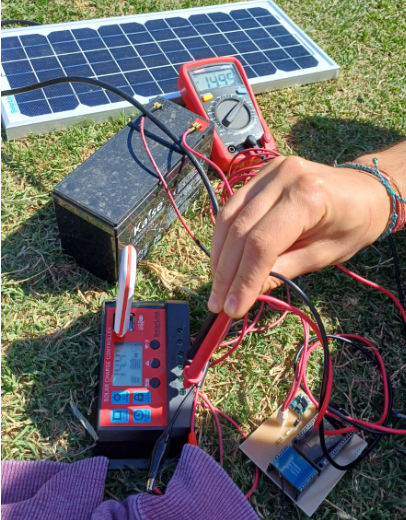
\includegraphics[scale=1]{./Figures/Pruebas/NodoAP-Pruebadistancia.PNG}
	\caption{Nodo Access Point sin su caja estanca.}
	\label{fig:NodoAp-PruebaDistancia}
\end{figure}

\begin{figure}[H]
	\centering
	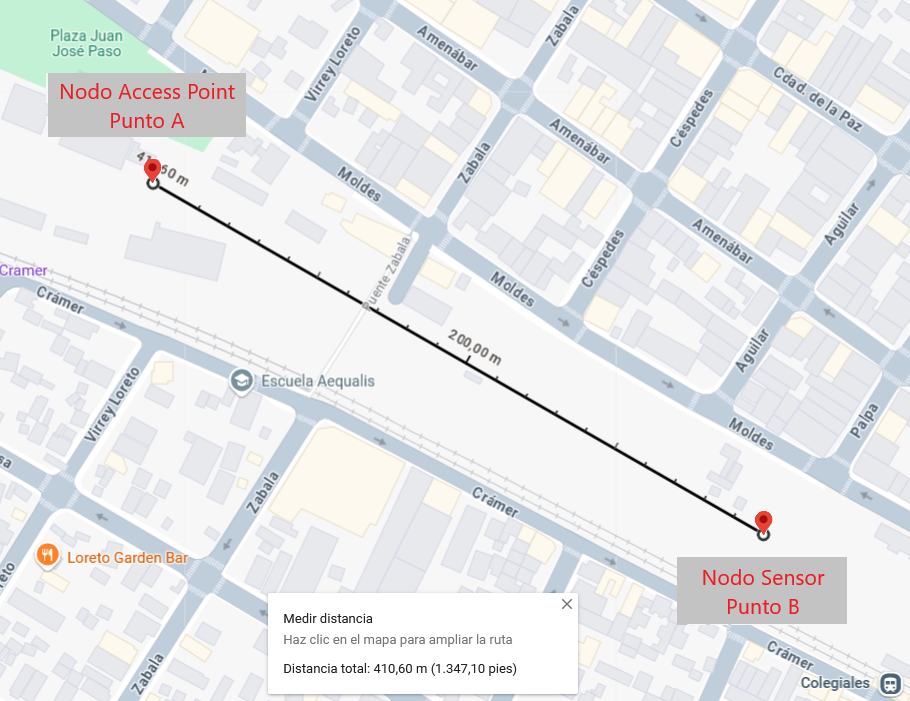
\includegraphics[scale=0.5]{./Figures/Pruebas/prueba_distancia_mapa.png}
	\caption{Visualización geolocalizada de los Nodos de la prueba.}
\label{fig:PruebaDistancia}
\end{figure}

Se consideró la prueba como un caso exitoso dado que a pesar de las condiciones radioeléctricas adversas (rebotes de la señal en los edificios cercanos, obstáculos entre los nodos, etc) los Nodos se comunicaron hasta los 410 metros, lo cual supera los requerimientos del proyecto. Esto quiere decir que en un verdadero campo abierto ideal la distancia máxima debería ser aun mayor.

En la Figura \ref{fig:PruebaDistanciaGrafana} se observan las mediciones que permitieron determinar el rango máximo, como así también el correcto funcionamiento del Nodo Access Point.

\begin{figure}[H]
    \centering
    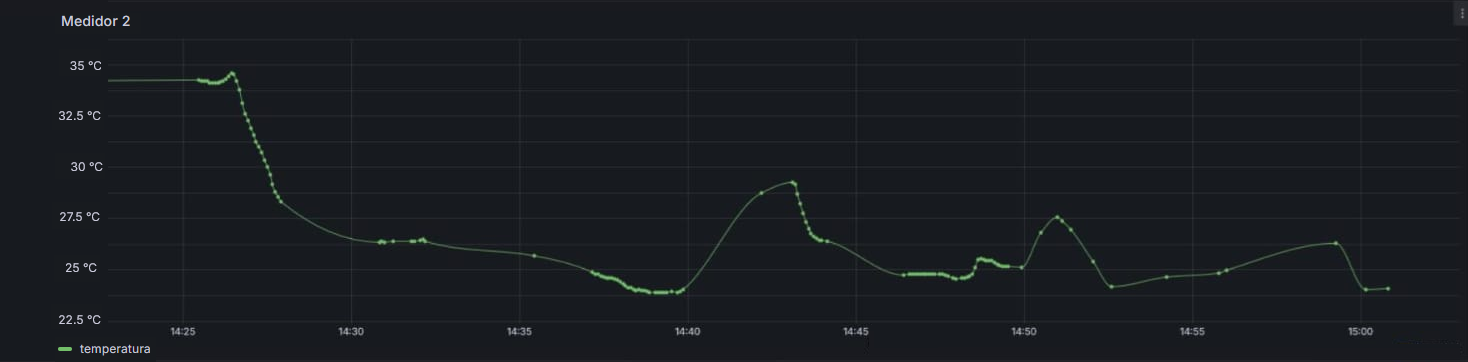
\includegraphics[width=1\linewidth]{Figures/Pruebas/prueba_distancia_grafana.png}
    \caption{Resultados de la prueba integral de distancia en Grafana.}
    \label{fig:PruebaDistanciaGrafana}
\end{figure}

Las distintas densidades de puntos se deben a que durante la prueba se cambiaron constantemente las orientaciones de las antenas. Cuanto menos espaciados están las mediciones mejor fue SNR y calidad de señal, y se observa que las últimas mediciones están muy espaciadas.

\subsection{Prueba Integral en Condiciones Reales}

En esta segunda prueba se verificó el funcionamiento en condiciones reales de los Nodos Sensores y Nodo  Access Point (enviando y recibiendo mediciones cada 1 hora).

Los dos Nodos Sensores se ubicaron en una misma habitación y el Nodo Access Point en un balcón con exposición a la luz solar de manera directa, de forma que el panel solar pueda cargar la batería. (Se entiende que en esta prueba no está maximizado el tiempo de exposición a la luz solar, y por lo tanto el tiempo de carga).

La figura \ref{fig:pruebas_grafana} muestra un tablero de Grafana dividido en dos secciones principales: la mitad superior presenta los gráficos correspondientes al Nodo Sensor número 2, mientras que la mitad inferior visualiza la información recopilada por el Nodo Access Point. Este diseño permite una comparación directa y simultánea de los datos recolectados por ambos nodos, facilitando el monitoreo integral del sistema.
Ambos nodos operaron durante mas de 28 horas sin interrupciones. 
Durante este período, el Nodo Access Point estuvo expuesto a luz solar durante medio día y operó durante otro medio día sin recargar la batería. A partir de estos resultados, se concluye que la capacidad del sistema para operar de manera continua durante más de 24 horas valida la sostenibilidad del ciclo de carga y descarga de la batería, garantizando su funcionamiento eficiente sin interrupciones.

\begin{figure}[H]
    \centering
    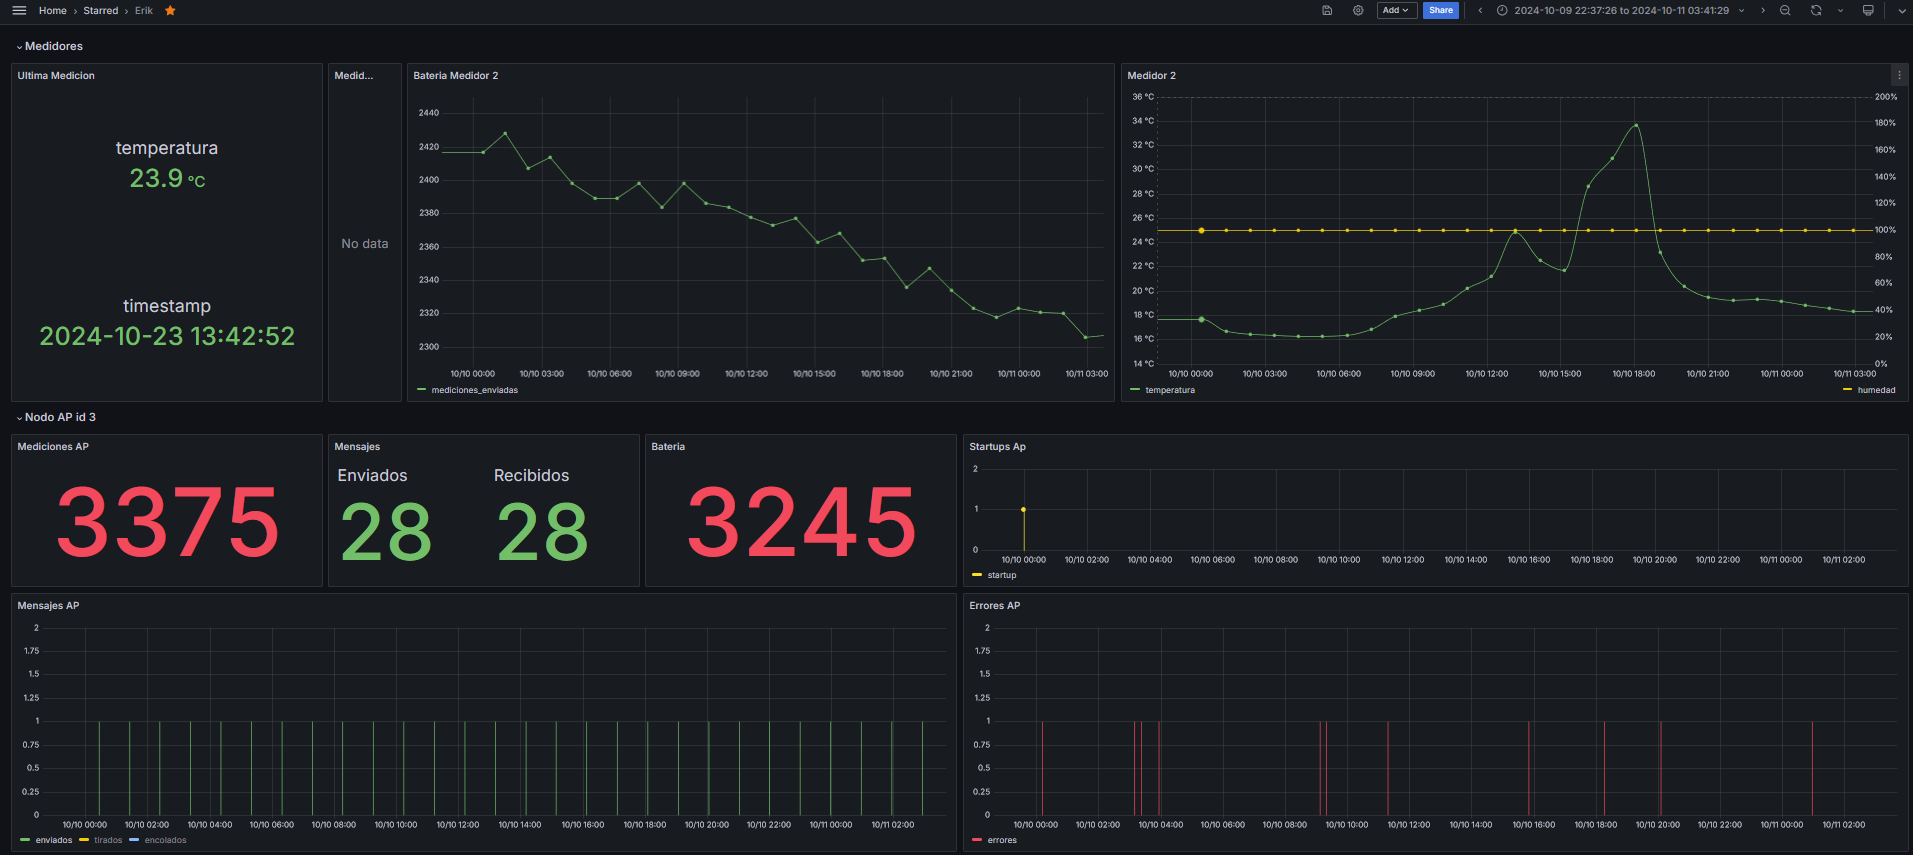
\includegraphics[width=1\linewidth]{Figures/Pruebas/pruebas_grafana.png}
    \caption{Resultados de la prueba integral vistas en Grafana.}
    \label{fig:pruebas_grafana}
\end{figure}

Por un lado, es importante destacar que el nivel de batería del Nodo Sensor 2 no ha sido procesado, por lo que no se presenta en una escala porcentual de 0 a 100, sino como el valor analógico medido.

Por otro lado, el Nodo Access Point demostró estabilidad en el sistema, al recibir y enviar todos los mensajes, así como al registrar una única medición de inicio (startup), lo que indica que, durante toda la prueba, no se produjo ningún reinicio.

Se observa que, en las horas de la tarde, con mayor exposición solar, la temperatura medida aumenta, especialmente entre las 15:00 y las 19:00 horas.

Finalmente, esta prueba reveló que, en un compost muy húmedo, el sensor alcanza una saturación y no muestra variaciones significativas durante períodos prolongados.
